\clearpage\subsubsection{Примечания}
\bigskip


\bigskip

\begin{enumerate}
\printpagenotes




\item \label{bkm:Ref474665714}К стр. \pageref{bkm:bm35}. — В немецком тексте
(как в издании Глокнера, так и в издании Лассона) вместо слова «nur» (лишь)
стоит «nun» (теперь). По-видимому, это опечатка.
\item \label{bkm:Ref474665735}К стр. \pageref{bkm:bm36}. — Немецкое слово
Quantitat (количество) образовано из латинского quantitas.
\item \label{bkm:Ref474665753}К стр. \pageref{bkm:bm37}. — Имеется в виду
юношеская философская работа Лейбница «О принципе индивидуализации»,
написанная им в 1663 г.
\item \label{bkm:Ref474665775}К стр. \pageref{bkm:bm38}. — {\em Кант},
Критика чистого разума, 2-е немецкое издание, стр.~449–450. Гегель
несколько перефразирует это место. Во 2-м издании перевода Лосского (Пгр.
1915) это место находится на стр.~263.
\item \label{bkm:Ref474665791}К стр. \pageref{bkm:bm39}. — В немецком тексте
вместо слов «nach denselben» (по ним,~т.~е. по этим моментам) стоят слова
«nach demselben» (по нему). По-видимому, это опечатка.
\item \label{bkm:Ref474665796}К стр. \pageref{bkm:bm40}. — В немецком тексте
вместо слова «quantitative» (количественное) стоит слово «qualitative»
(качественное). По-видимому, это опечатка.
\item \label{bkm:Ref474665804}К стр. \pageref{bkm:bm41}. — Имеются в виду
Шеллинг и его последователи в натурфилософии.
\item \label{bkm:Ref474665813}К стр. \pageref{bkm:bm42}. — Цитата взята с
предпоследней страницы «Критики практического разума» Канта.
Непосредственно перед этим находится известное место, начинающееся словами:
«две вещи наполняют душу всегда новым удивлением и благоговением... — это
звездное небо над нами и моральный закон внутри нас» (См. {\em Кант},
Критика практического разума, пер. Соколова, Спб. 1897, стр.~191).
\item \label{bkm:Ref474665836}К стр. \pageref{bkm:bm43}. — О «не-я» как о
«толчке» (Anstoss) Фихте говорит в начале третьей части своей книги «Основа
общего наукоучения» (1794 г.). В русском переводе «Избранных сочинений И.
Г. Фихте» (т.~I, М.~1916) о «толчке» говорится на стр. 226–227.
\item \label{bkm:Ref474665876}К стр. \pageref{bkm:bm44}. — Имеется в виду
шеллингова «система абсолютного тождества», как она развита главным образом
в сочинении Шеллинга «Изложение моей системы философии» (1801 г.).
\item \label{bkm:Ref474665904}К стр. \pageref{bkm:bm45}. — Намек на
сатирическое стихотворение Шиллера «Die Philosophen», 16-е двустишие
которого (под заголовком: «Вопрос о праве») гласит:\newline
«Jahrelang schon bedien ich meiner Nase zum Riechen;\newline
Hab ich denn wirklich an sie auch ein erweisliches Recht?»\newline
(«Уже в течение многих лет я пользуюсь своим носом для нюханья, но имею ли я
и в самом деле право на это —~право, которое можно было бы доказать и
обосновать?»).
\item \label{bkm:Ref474665953}К стр. \pageref{bkm:bm46}. — В немецком тексте
вместо «которого» (dessen) стоит «которой» (deren). По-видимому, это
опечатка.
\item \label{bkm:Ref474665962} К стр. \pageref{bkm:bm47}. — Фигуру двух
неконцентричных кругов (см. рис.), заимствованную у Декарта («Принципы
философии», часть~II, §~33), Спиноза изобразил, в виде виньетки, на
титульном листе своего геометрического изложения «Принципов философии
Декарта» (вышло в Амстердаме в 1663 г.), а не «Этики», как ошибочно
утверждает Гегель.
\begin{center}
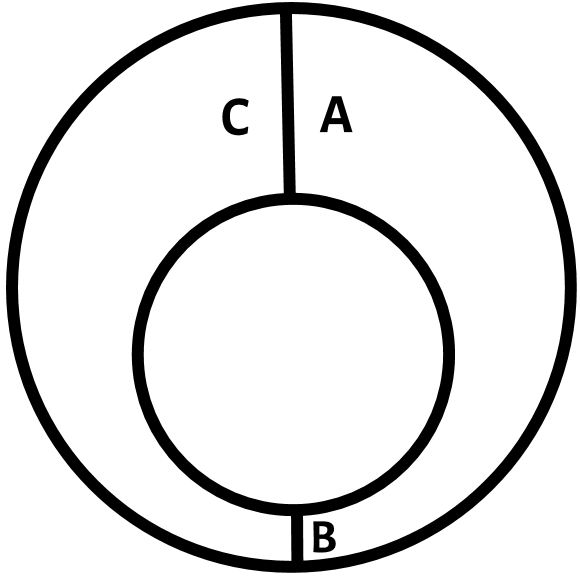
\includegraphics[width=1.25in,height=1.25in]{hegel-img002.png}
\end{center}
\item \label{bkm:Ref474665968}К стр. \pageref{bkm:bm48}. — Гегель дает здесь
в весьма вольном переводе и с перестановкой отдельных предложений
рассуждения Спинозы о бесконечном множестве неравных расстояний между двумя
неконцентричными окружностями (см. Спиноза, Переписка, М.~1932, стр.~78).
Конец приводимой Гегелем цитаты у Спинозы гласит: «...природа этой вещи не
может быть выражена никаким числом».
\item \label{bkm:Ref474666121}К стр. \pageref{bkm:bm49}. — В немецком тексте
вместо  стоит , а вместо  $(x+i)^n$ напечатано . Явная опечатка.
\item \label{bkm:Ref474666136}К стр. \pageref{bkm:bm50}. — Проверка с
помощью числа девять —~громоздкий искусственный прием, в настоящее время
вышедший из употребления, ввиду своей непрактичности.
\item \label{bkm:Ref474666147}К стр. \pageref{bkm:bm51}. — т.~е. «ведь эти
члены не будут иметь {\em никакого} значения» (или: «{\em никакого}
веса», «{\em никакой} силы»).
\item \label{bkm:Ref474666169}К стр. \pageref{bkm:bm52}. — См. стр.
\pageref{bkm:bm52a}–\pageref{bkm:bm52b}.
\item \label{bkm:Ref474666189}К стр. \pageref{bkm:bm53}. — Под
«Entwicklungspotenz» Гегель, как видно из этого места, а также из первого
абзаца следующего примечания («Еще другие формы, находящиеся в связи с
качественной определенностью величины», — стр. \pageref{bkm:bm53a}),
понимает то же самое, что в других местах он обозначает терминами:
«Entwicklungsglied» (член ряда, получающегося при разложении двучлена  по
формуле Ньютона), «Entwicklungsfunktion» (функция, получающаяся в
результате разложения в ряд, — «функция развертывания», как иногда
приходится переводить это выражение: см. напр. стр. \pageref{bkm:bm53b}),
«die Funktion der Potenzierung» (функция возвышения в степень),
«abgeleitete Funktion» (производная функция,— обычный в математике термин
для обозначения того, о чем здесь идет речь у Гегеля). Употребляя для
обозначения производной функции несколько странное выражение
«Entwicklungspotenz», Гегель, по-видимому, хочет подчеркнуть существенное
значение того обстоятельства, что дело идет тут именно о {\em степенных}
функциях, о разложении по {\em степеням}, о том, что интересующая нас
переменная величина {\em имеет степень выше первой} (см. выше, стр.
\pageref{bkm:bm53c}). Поэтому как первоначальную, так и производную функцию
Гегель называет «{\em степенными} функциями» (Potenzenfunktionen).
\end{enumerate}
В связи с этим нельзя не привести отзыв Энгельса. В письме Марксу от 18
августа 1881 г. Энгельс, говоря о математических рукописях Маркса, замечает
по поводу математических примечаний Гегеля: «Старик Гегель... вполне
правильно угадал, говоря, что дифференцирование в виде основного условия
требует, чтобы обе переменных имели различные степени и чтобы по меньшей
мере одна из них была во второй или $\frac 1 2$-й степени. Теперь мы уже знаем
почему». ({\em Маркс} и {\em Энгельс}, Соч., т.~XXIV, стр.~531–532).

\begin{enumerate}
\item \label{bkm:Ref474666244}К стр. \pageref{bkm:bm54}. — См. прим.
\ref{bkm:Ref474666189}.
\item \label{bkm:Ref474666256}К стр. \pageref{bkm:bm55}. — В немецком тексте
вместо «verglichen» стоит «vergleichen». По-видимому, это опечатка.
\item \label{bkm:Ref474666305}К стр. \pageref{bkm:bm56}. — Здесь слово «нуль»
употребляется Гегелем в фигуральном смысле —~в том смысле, что сторона
обратного отношения перестает быть стороной отношения, если она становится
равной показателю. В математическом же смысле, если мы возьмем обратное
отношение, показателем которого является произведение членов отношения  и
приравняем один из членов отношения этому произведению (например, ), то
другой член отношения будет не нулем, а единицей (у = 1). В арифметическом
обратном отношении (о котором здесь у Гегеля еще нет речи и формулой
которого является $х+у=С$), действительно, если $х=C$,
то $у=0$.
\item \label{bkm:Ref474666541}К стр. \pageref{bkm:bm57}. — В немецком тексте
вместо «keine» (никакой) стоит «eine». По-видимому, это опечатка.
\item \label{bkm:Ref474666560}К стр. \pageref{bkm:bm58}. — В издании Лассона
эта часть фразы дается по 1-му изданию «Науки логики», где эта фраза
гласит: «И вот определенное количество, которое отныне уже не есть
безразличное или внешнее определение, а дано так, что оно вместе с тем
снято как такое определение...» и~т.~д.
\item \label{bkm:Ref474666566}К стр. \pageref{bkm:bm59}. — Гегель имеет в
виду философию Шеллинга.
\item \label{bkm:Ref474666577}К стр. \pageref{bkm:bm60}. — Английское слово
«фут» означает прежде всего «нога, ступня», а затем уже «фут» в смысле меры
длины, приблизительно соответствующей длине ступни человека
(30,5~{\em см}). То же самое имеет место и в немецком языке со словом
«Fuss».
\item \label{bkm:Ref474666643}К стр. \pageref{bkm:bm61}. — Слово «правило»
(die Regel) Гегель употребляет здесь в смысле «мерило», «масштаб», «норма»,
«образцовая или указная мера» (Massregel, Richtmass). В XVIII в. слово
«Regel» иногда употреблялось в смысле линейки с делениями. Гегель,
по-видимому, и намекает на это старинное значение.
\item \label{bkm:Ref474666655}К стр. \pageref{bkm:bm62}. — Гегель
рассматривает здесь понятие физической {\em константы},~т.~е. того
эмпирического коэффициента, который в той или иной форме входит в уравнения
механики и физики. В качестве примера такой константы Гегель в следующей
фразе приводит величину $а$ в уравнении движения падения тел 
$s=at^2$. Гораздо чаще формулу движения падения тел
выражают уравнением $s=\frac 1 2 gt^2$, где константа
$g$ (постоянное для данного географического пункта ускорение силы
тяжести) равна приблизительно $9,8 \text{\em м}$ (в качестве единицы времени
берется при этом секунда). Следовательно, величина $а$ в уравнении
равна приблизительно $4,9 \text{\em м}$. Впрочем, надо сказать, что величина
$а$ или $g$, входящая в формулу движения падения тел, может
быть названа константою лишь в весьма относительном смысле. Дело в том, что
сама она изменяется с изменением расстояния от центра земного шара (а также
от расположения тяжелых масс на земной поверхности вблизи того места, где
производятся опыты с падением тел). Но так как эти изменения весьма
незначительны в тех случаях падения тел, которые рассматриваются в
элементарной механике (т.~е. в тех случаях, где расстояния, проходимые
падающим телом, незначительны по сравнению с длиной земного радиуса, причем
опыты производятся в одном и том же месте земной поверхности), то ими
вполне можно пренебречь.
\item \label{bkm:Ref474666676}К стр. \pageref{bkm:bm63}. — Здесь, как и в
предыдущем разделе «Мера как ряд отношений мер», Гегель имеет в виду учение
шведского химика Торберна Бергмана (1735–1784) о количественном выражении
сродства между основаниями и кислотами. Бергман предполагал, что одно и то
же количество какого-нибудь химического основания тем больше требует
кислоты для своего насыщения или нейтрализации, чем больше у них сродства
друг с другом. Он нашел, что для насыщения, например, 100 весовых частей
едкого кали требуется 78,5 весовых частей серной кислоты, или 64 весовых
частей азотной кислоты, или 51,5 весовых частей соляной кислоты и~т.~д.;
для насыщения же 100 весовых частей едкого натра нужно 177 весовых частей
верной кислоты, либо 135,5 весовых частей азотной кислоты, либо 125 весовых
частей соляной кислоты и~т.~д. В том и другом случае {\em порядок}
кислот остается {\em один и тот же}. Получается некоторой ряд пропорций
или мер насыщения (нейтрализации), который, по Гегелю, и характеризует
собой специфическую природу исследуемого вещества, выступающего в качестве
{\em противочлена} этого ряда. Учение Бергмана о химическом сродстве и
его количественном выражении было господствующей теорией в последней
четверти XVIII в. В начале XIX в. появилась новая теория химического
сродства, связанная с именем французского химика Клода Бертоллэ
(1748–1822), в значительной мере направленная против теории Бергмана.
Бертоллэ считал, что, наоборот, чем меньшее количество вещества $А$
требуется для нейтрализации вещества $В$, тем больше сродство между
ними. Кроме того, также и числовые значения мер насыщения, найденные
Бергманом, оказались при более тщательных экспериментах весьма неточными.
Сочинения Бергмана были изданы в немецком переводе в 1782–1799 гг. и были
широко известны в Германии. Между прочим, от Бергмана идет термин
«attractio electiva» (избирательное притяжение), который в немецком
переводе был передан термином «Wahlverwandtschaft» (избирательное
сродство), употребляемым здесь у Гегеля для обозначения одной из категорий
меры. Подробнее о теориях Бергмана и Бертоллэ см. у {\em Hermann Корр},
Geschichte der Chemie, Neudruck der Originalausgabe, Leipzig 1931, Bd. II,
S. 297–324, откуда и взяты вышеприведенные сведения. — Что касается
«избирательного сродства», как химической категории, то принцип этого
сродства был сформулирован еще задолго до Бергмана французским химиком
Этьеном Жоффруа (1672–1731), который в 1718 г. выставил следующее
положение: «Всякий раз, когда мы имеем соединение двух веществ, обладающих
склонностью соединяться друг с другом, если к этому соединению
примешивается третье вещество, имеющее более сильное сродство с одним из
первых двух, то это третье вещество соединяется с ним, отбивая его от
другого» (цитировано у Коппа, стр.~296 второго тома),~т.~е. указанное
третье вещество разлагает первоначально данное соединение, соединяясь с
одним из компонентов и вытесняя из соединения другой компонент.
\item \label{bkm:Ref474666698}К стр. \pageref{bkm:bm64}. — Имеется в виду
учение Бергмана (см. предыдущее примечание).
\item \label{bkm:Ref474666706}К стр. \pageref{bkm:bm65}. — «Учебник химии»
Берцелиуса вышел в трех томах в 1808–1828 гг.
\item \label{bkm:Ref474666715}К стр. \pageref{bkm:bm66}. — Гегель неправ:
причиной остановки маятника является не сила тяжести, а трение в том месте,
где маятник прикреплен или привязан, а также и сопротивление воздуха (или
какой-нибудь другой среды, в которой качается маятник).
\item \label{bkm:Ref474666719}К стр. \pageref{bkm:bm67}. — Немецкий текст
здесь испорчен. Перевод сделан на основе конъектуры Б. Г. Столпнера,
предлагающего вместо «eintretender qualitativer Bestimmtheit» читать
«eintretende qualitative Bestimmtheit». Лассон предлагает другую
конъектуру, вставляя перед указанными словами слова «ein Unterschied». В
этом случае надо было бы перевести эту фразу следующим образом: «Если,
таким образом, различие химического сродства, в противоположность
избирательному сродству, точно устанавливается в некотором ряде
количественных отношений, как различие появляющейся качественной
определенности...» и~т.~д.
\item \label{bkm:Ref474666725}К стр. \pageref{bkm:bm68}. — Имеются в виду
электрохимические теории английского химика Дэви (1778—1829) и шведского
химика Берцелиуса (1779–1848), явившиеся крупным шагом вперед в развитии
химии. Гегель недооценивал их значение, так же, как он недооценивал
прогрессивное значение химических теорий Бертоллэ.
\item \label{bkm:Ref474666740}К стр. \pageref{bkm:bm69}. — Выражение
«индифференция» (неразличенность, безразличие) было употреблено Шеллингом в
его вышедшей в 1801 г. работе «Изложение моей системы философии» для
обозначения «абсолютного тождества» субъекта и объекта. «Совершенная
неразличенность (totale Indifferenz) субъективного и объективного» —~таково
было основное понятие этой фазы философского развития Шеллинга. В
дальнейшем Гегель подробно рассматривает шеллинговскую концепцию
«индифференции как обратного отношения между ее факторами» и подвергает ее
имманентной критике, вскрывая ее «всестороннюю противоречивость». По учению
Шеллинга абсолютное представляет собою неподвижное тождество, полнейшую
неразличенность, совершенное безразличие двух факторов: субъективного и
объективного. Всякое же дифференцирование состоит лишь в количественном
перевесе одного из этих двух факторов над другим, причем «вечным основанием
и опорою всех количественных различий субъективного и объективного служит
их совершенная индифференция, составляющая форму абсолютного тождества,
форму их бесконечного бытия» (см. {\em Куно Фишер}, Шеллинг, его жизнь,
сочинения и учение, пер. H. Лocского, Спб. 1905, стр. 590). О шеллинговой
системе «абсолютного тождества» Гегель упоминал также и выше, на
стр.~\pageref{bkm:bm69a}. Ср. прим.~\ref{bkm:Ref474665876} к этому месту.
\item \label{bkm:Ref474666761}К стр. \pageref{bkm:bm70}. — См. предыдущее
примечание.
\item \label{bkm:Ref474666774}К стр. \pageref{bkm:bm71}. — В первом издании
«Науки логики» (1812) здесь стояла еще следующая фраза, выпущенная Гегелем
в 1831 г., когда он готовил второе издание: «Этот вопрос я осветил в моей
более ранней диссертации, где я доказал несостоятельность этого различения
и построенных на нем объяснений». Имеется в виду «Философская диссертация
об орбитах планет» (1801) Возможно, что Гегель выпустил эту ссылку на свою
диссертацию потому, что в ней, между прочим, доказывалось, что между
Юпитером и Марсом не может быть никаких планет, между тем как еще в 1801 г.
была открыта малая планета Церера, расположенная как раз между Юпитером и
Марсом.
\item \label{bkm:Ref474666782}К стр. \pageref{bkm:bm72}. — Это не совсем
так. Как уже было упомянуто в примечании \ref{bkm:Ref474665489}{}-м, Гегель
в значительной мере произвольно толковал философию Спинозы, приписывая ей
акосмизм (отрицание мира) и идеализм. В этом отношении он шел по стопам
Шеллинга, использовавшего некоторые элементы спинозизма для построения
своей идеалистической философии «абсолютного тождества». В действительности
же между материалистом Спинозой и объективным идеалистом Шеллингом огромная
принципиальная разница, и эта-то разница как раз и смазывается в
гегелевской трактовке спинозизма.
\item \label{bkm:Ref474666794}К стр. \pageref{bkm:bm73}. — См. «Учение о
бытии», стр. \pageref{bkm:bm73a}—\pageref{bkm:bm73b}.
\item \label{bkm:Ref474666798}К стр. \pageref{bkm:bm74}. — В немецком тексте
вместо sie (т.~е. Negation) стоит es. По-видимому, это опечатка.
\item \label{bkm:Ref474666813}К стр. \pageref{bkm:bm75}. — См. примечание
\ref{bkm:Ref474665836}.
\item \label{bkm:Ref474666829}К стр. \pageref{bkm:bm76}. — См.
{\em Кант}, Критика способности суждения, пер. Н. Соколова, Спб. 1898,
стр. 16—17.
\item \label{bkm:Ref474666833}К стр. \pageref{bkm:bm77}. — Здесь кончается
выписка из «Критики способности суждения» (стр. XXVI немецкого издания 1799
г., стр.~16 русского перевода).
\item \label{bkm:Ref474666843}К стр. \pageref{bkm:bm78}. — Гегель имеет в
виду Шеллинга и его последователей. Шеллинг начиная с 1800 г., когда он
выпустил свою «Систему трансцендентального идеализма», выдвигает в качестве
«органа всякого трансцендентального мышления» «интеллектуальную интуицию»,
как непосредственное созерцание абсолютного, целиком противоположное
рассудочному познанию и совершенно оторванное от него. Против шеллинговой
«интеллектуальной интуиции» Гегель впервые выступил в начале 1807 г в
предисловии к «Феноменологии духа». В своих «Лекциях по истории философии»
Гегель дает более развернутую критику Шеллинга и его поклонников. Особенно
резко он отзывается об этих последних. «Вся эта тенденция, — говорит он об
антинаучном характере философских упражнений шеллингианцев, —
противопоставляет себя прежде всего {\em рефлективному мышлению}, или,
иначе сказать, такому движению рассуждения, которое держится фиксированных,
прочных, неподвижных понятий. Но вместо того чтобы оставаться в области
понятия и познать его как беспокойное «я», они впали в противоположную
крайность покоящегося созерцания, непосредственного бытия, неподвижного «в
себе» и полагают, что этот недостаток, эта неподвижность, исправляется
глядением и что это глядение они превращают в интеллектуальное, определяя
его в свою очередь посредством какого-нибудь фиксированного понятия»
({\em Гегель}, Лекции по истории философии, кн.~III. М.—Л. 1936,
стр.~511).
\end{enumerate}
Самое слово «рефлексия» Гегель употребляет в различных значениях, притом
так, что одно значение незаметно переходит у него в другое или даже
совмещается с другим. Латинское слово «reflexio» означает «загибание назад,
отклонение назад, отражение» (света, звуковой волны, брошенного во
что-нибудь предмета). В новых языках это слово наряду с этим значением
«отражения» приобрело еще значение «размышления, обдумывания, рассуждения,
соображения, рассудительности» (мысль как бы оборачивается на самоё себя,
отражается в себя самоё). У Гегеля рефлексия берется то в объективном, то в
субъективном смысле. При этом Гегель, как объективный и абсолютный
{\em идеалист}, понимает объективную рефлексию не в смысле взаимного
отражения сторон или моментов материального предмета друг другом или друг в
друге и не в смысле обратного их отражения в себя самих, а в смысле
взаимного отражения между определениями понятия как такового или в смысле
обратного отражения какого-нибудь понятийного определения внутрь себя
самого («рефлексия в себя»). Субъективную же рефлексию Гегель, как
идеалист, берет не в смысле гносеологического отражения объективно-реальной
материальной действительности в человеческом или животном сознании, а в
смысле рассудочного оперирования абстрактными категориями чистой мысли.
Рефлексия рассудка подвергается у Гегеля уничтожающей критике в том случае,
если она выступает с претензией на полное, завершенное, абсолютное
познание. Но вместе с тем Гегель решительно защищает эту рефлексию рассудка
как необходимый момент в диалектическом развитии познания (против Шеллинга
и шеллингианцев, против Якоби и против романтиков). Рефлексия в себя и
рефлексия в другое (притом не в другое вообще, а в «{\em свое} другое»)
составляют, по Гегелю, характерную черту категорий сущности (которая ведь
представляет собою «абсолютное опосредствование с собою»), точно так же как
переход от одного к другому был характерной чертой категорий бытия (где
господствует непосредственность), а развитие или развертывание
(Entwickelung) будет характерной чертой категорий понятия (где имеет место
единство непосредственного и опосредствованного).

В теснейшей связи с выражением «рефлексия» Гегель употребляет выражение
«Scheinen», имеющее у него опять-таки специфически-метафорическое значение.
«Das Scheinen» означает у Гегеля «свечение, мерцание, отблеск» (например,
Гегель говорит, что положительное «светится» в отрицательном, а
отрицательное —~в положительном; см. в тексте стр. \pageref{bkm:bm78a}).
Иногда Гегель приводит выражение «Scheinen» в прямою связь с термином
«Schein» (видимость, кажимость), и тогда «das Scheinen» приходится
переводить словами «свечение видимостью» (в себе самом или в своем другом),
или «излучение видимости» (в себя самого или в свое другое).

\begin{enumerate}
\item \label{bkm:Ref474666865}К стр. \pageref{bkm:bm79}. — В немецком тексте
(как в издании Глокнера, так и в издании Лассона) вместо слова
«положительным» стоит слово «отрицательным». По-видимому, это опечатка.
\item \label{bkm:Ref474666880}К стр. \pageref{bkm:bm80}. — В немецком тексте
наоборот: «+~а раз –~а». По-видимому, это опечатка.
\item \label{bkm:Ref474666891}К стр. \pageref{bkm:bm81}. — Об игре слов в
немецком выражении «zu Grunde gehen», как его употребляет Гегель, см.
замечания Энгельса в письмах Конраду Шмидту от 1 ноября 1891 г. и от 4
февраля 1892 г. ({\em Маркс} и {\em Энгельс}, Письма, под ред.
Адоратского, изд. 4-е, М.—Л. 1931, стр. 393–394).
\item \label{bkm:Ref474666904}К стр. \pageref{bkm:bm82}. — Слово «этиология»
(от греческого «aitia» —~причина, начало, основание) означает учение о
причинах, указание причин или оснований для тех или иных явлений.
\item \label{bkm:Ref474666911}К стр. \pageref{bkm:bm83}. — Лассон считает,
что придаточное предложение «что растение имеет свое основание в
производящей растения силе» попало сюда по ошибке и должно быть поставлено
двумя строчками выше, после слов «я скажу, что оно есть растение».
Стилистически такая перестановка улучшает конструкцию всей этой фразы, но
логический смысл заставляет предпочесть тот текст, какой дается в издании
Глокнера. С этого текста и сделан перевод этой фразы с добавлением слов
«того предложения» перед приведенным выше придаточным предложением.
\item \label{bkm:Ref474666923}К стр. \pageref{bkm:bm84}. — т.~е. по-своему,
по-разному.
\item \label{bkm:Ref474666940}К стр. \pageref{bkm:bm85}. — См. «Учение о
бытии», стр. \pageref{bkm:bm85a}–\pageref{bkm:bm85b}.
\item \label{bkm:Ref474667017}К стр. \pageref{bkm:bm86}. — В русском
переводе под ред. Радлова ({\em Гегель}, Феноменология духа, Спб. 1913)
это место находится на стр. 72—74 (в главе «Сила и рассудок, явление и
сверхчувственный мир»).
\item \label{bkm:Ref474667030}К стр. \pageref{bkm:bm87}. — В немецком
тексте: «das Relative eines Ändern». По-видимому, это опечатка вместо: «das
Relative seines Ändern».
\item \label{bkm:Ref474667041}К стр. \pageref{bkm:bm88}. — См. часть первая,
стр. \pageref{bkm:bm88a}–\pageref{bkm:bm88b}.
\item \label{bkm:Ref474667057}К стр. \pageref{bkm:bm89}. — В немецком
тексте: «in derselben». По-видимому, это опечатка вместо: «in demselben».
\item \label{bkm:Ref474667072}К стр. \pageref{bkm:bm90}. — Ср. замечание
Энгельса о том, что «сила имеет точно такую же величину, как и ее
проявление во-вне, ибо в них обоих совершается {\em одно и то же
движение}» ({\em Engels}, Herrn E. Dührings Umwälzung der Wissenschaft.
Moskau —~Leningrad 1935, S.~64).
\item \label{bkm:Ref474669620}К стр. \pageref{bkm:bm91}. — См. примечания
\ref{bkm:Ref474665489} и \ref{bkm:Ref474666782}.
\item \label{bkm:Ref474669634}К стр. \pageref{bkm:bm92}. — Это не точно. 4-я
дефиниция первой части «Этики» гласит: «Под атрибутом я разумею то, что
интеллект мыслит о субстанции, как составляющее ее сущность». Из
сопоставления этой дефиниции с рядом других мест из «Этики» и из
«Переписки» Спинозы видно, что атрибуты, но учению Спинозы, не только
{\em мыслятся} интеллектом как составляющие сущность субстанции, но и
действительно «выражают, раскрывают и составляют вечную сущность и вечное
существование» субстанции безотносительно к интеллекту (см., например,
доказательства теоремы 19-й и 20-й первой части «Этики» и письмо 2-е).
Субстанция, говорит Спиноза, {\em имеет} атрибуты (доказательство
теоремы 16-й первой части «Этики»).
\item \label{bkm:Ref474669669}К стр. \pageref{bkm:bm93}. — Абсолютная
необходимость слепа потому, что она равносильна абсолютной случайности, как
это более определенно намечается Гегелем в непосредственно следующих за
этим рассуждениях, содержащих элементы диалектической критики категории
абсолютной необходимости. Если все одинаково абсолютно-необходимо, если
все, что существует, существует только потому, что оно существует, не имея
для своего существования никаких других оснований, то это значит, что все
абсолютно случайно. Здесь получается {\em непосредственное} или, как
выражается Гегель, намекая, по-видимому, на Шеллинга (а также, без сомнения,
и на метафизический детерминизм Спинозы), «{\em абсолютное}» тождество
сущности и бытия, возможности и действительности, необходимости и
случайности —~такое тождество, где отсутствует самодвижение, где имеется
лишь «рефлексия в себя» без «рефлексии в другое». Сама сущность выступает
здесь в форме «бытия», в форме простой непосредственности, простого факта.
Подобно тому, как ночью, согласно немецкой поговорке, «все коровы черны»
(или, согласно русской поговорке, «все кошки серы»), так и в «одноцветном»
абсолюте Шеллинга все совершенно одинаково {\em по своей форме}, все
различия между отдельными категориями стерты, растворены в «пустой бездне»
({\em Гегель}, Феноменология духа, предисловие, стр. 12 в немецком
издании Лассона, Лейпциг 1921, или стр. 7 в русском переводе под ред.
Радлова, Спб. 1913). Что касается специально абсолютной необходимости, то
возможность абсолютно-необходимого и его действительность непосредственно
совпадают именно потому, что все вещи и все события рассматриваются на
данном этапе как {\em одинаково} необходимые, как необходимости
{\em одного и того же порядка}. Ср. классические формулировки Спинозы:
«Из необходимости божественной природы должно следовать бесконечно многое
бесконечно-многими способами,~т.~е. все то, что может стать объектом
бесконечного интеллекта» («Этика», ч.~I, теор.~16); «из бесконечной природы
бога все всегда следует по одной и той же необходимости, точно таким же
образом, как из природы треугольника от века и до века следует, что его три
угла равны двум прямым» (там же, схолия к теор. 17). По Спинозе, все
отдельные вещи одинаково необходимы, но вместе с тем все они одинаково
случайны (см. королларий к теор. 31 второй части и дефиницию 3-ю четвертой
части).
\end{enumerate}
В своем гениальном отрывке о «Случайности и необходимости» Энгельс, отмечая
заслуги Гегеля по части диалектической трактовки категорий необходимости и
случайности, дает замечательный по своей глубине и ясности диалектический
анализ и диалектическую критику точки зрения абсолютной необходимости,
которую он характеризует как «механический детерминизм, который на словах
отрицает случайность в общем, чтобы на практике признать ее в каждом
отдельном случае» («Диалектика природы», изд. 1936 г., стр. 109).
Механический детерминизм, указывает Энгельс, «деградирует необходимость до
уровня случайности» (там же, стр. 108).

Известное положение Гегеля о том, что «слепа необходимость лишь постольку,
поскольку она не постигается в понятии» ({\em Гегель}, Собр. соч., т. I,
стр. 248; ср. {\em Энгельс}, Анти-Дюринг, гл. XI первого раздела),
нисколько не противоречит его трактовке абсолютной необходимости в
рассматриваемом месте, ибо абсолютная необходимость, провозглашаемая
механическим детерминизмом, по самому существу своему не может быть
объектом конкретного, адэкватного познания, не может быть «постигнута в
понятии». Поэтому Гегель и говорит, что в стадии абсолютной необходимости
(или, что то же самое, в стадии абсолютной действительности, абсолютного
факта) необходимость «заперта» в бытии, что она «боится света». В
дальнейшем, а именно при переходе от «Сущности» к «Понятию», необходимость
«раскроется» (ср. в тексте стр. \pageref{bkm:bm93a}) и тем самым перестанет
быть «слепой».

\begin{enumerate}
\item \label{bkm:Ref474669698}К стр. \pageref{bkm:bm94}. — Это предисловие
предпослано IV т. Собрания сочинений Гегеля, изданного вскоре после его
смерти его учениками, — тому, содержащему 2-ю часть «Науки логики»
—~«Учение о сущности».
\item \label{bkm:Ref474655210}К стр. \pageref{bkm:bm95}. — Имеется в виду
изречение Лессинга о том, что если бы бог предложил ему выбор между
готовой, законченной, чистой истиной и вечно живым стремлением к ней,
стремлением, связанным с постоянными ошибками и заблуждениями, то он выбрал
бы последнее. См. Lessings Philosophie, hrsg. von Paul Lorenz, Leipzig
1909, S. 106.
\end{enumerate}

\bigskip


\bigskip
